\newcommand{\ONEtitle}{XXXXXX}
\newcommand{\ONEteam}{XXXXX}
\newcommand{\ONEdate}{Abc XX, 2020}
\newcommand{\ONEauthor}{Xxxx XXXXXXX}
\newcommand{\ONEchecker}{}
\newcommand{\ONEserial}{AR-XXXXXXXX-XXX}
\newcommand{\ONEedits}{
    \begin{tabular}{|c|c|c|C{10cm}|}
		\hline
		\rowcolor{lightgray}
		Ed. & Rev. & Date & Modifications\\
		\hline
		1 & 0 & XX/XX/2019 & Document creation\\
		\hline  
		&  & & \\ 
		\hline    
		&  & & \\ 
		\hline
		&  & & \\ 
		\hline
		&  & & \\ 
		\hline
		&  & & \\ 
		\hline
		&  & & \\ 
		\hline   
	\end{tabular}
}




\documentclass[12pt, a4paper, openright]{report}
\usepackage[T1]{fontenc}
\usepackage[utf8]{inputenc}
\usepackage[english]{babel} %Met en français
\usepackage[top=1.5cm, bottom=2.5cm, left=2.5cm, right=2.5cm]{geometry} %changement du cadre
\usepackage{setspace} %Modification des interlignes
\usepackage{graphicx} %insertion d'image
\usepackage{multirow}
\usepackage{booktabs} %Excel2LaTeX
\usepackage{tikz}
\usepackage{amsmath}
\usepackage{amsfonts}
\usepackage{fancyhdr}
\usepackage{lastpage}
\usepackage{array}
\newcommand{\PreserveBackslash}[1]{\let\temp=\\#1\let\\=\temp}
\newcolumntype{C}[1]{>{\PreserveBackslash\centering}p{#1}}
\usepackage{lmodern}
\usepackage{mathtools, bm}
\usepackage{amssymb, bm}
\usepackage{libertine}
\usepackage{listings}
\usepackage{pdflscape}
\usepackage{indentfirst}
\setlength\parindent{2em}
\usepackage{wrapfig}
\usepackage{eurosym}
\usepackage{url}
\usepackage{hyperref}
\usepackage{tabto}
\hypersetup{
    colorlinks=true,
    linkcolor=blue,
    filecolor=magenta,      
    urlcolor=cyan,
}
\lstset{
  basicstyle=\ttfamily,
  columns=fullflexible,
  frame=single,
  breaklines=true,
  postbreak=\mbox{\textcolor{red}{$\hookrightarrow$}\space},
}
\usepackage{titletoc}
\usepackage[demo]{adjustbox}
\usepackage{xcolor}
\usepackage{tikzpagenodes} 
\usepackage{tabularx,colortbl}              
\usetikzlibrary{calc}        
\usepackage{lipsum}           
\usetikzlibrary{calc}
\usepackage{ifthen}
\usepackage[contents={},opacity=1,scale=1.485]{background}
\definecolor{bleuONE}{RGB}{0,112,192}
\definecolor{vertONE}{RGB}{112, 173, 71}
%%%%%%%%%%%%%%%%%%%%%%%%%%%
% Définition des couleurs %
%%%%%%%%%%%%%%%%%%%%%%%%%%%
\fancypagestyle{pagedegarde}{%
	\fancyhf{}
	\fancyhead[LO]{%
		\begin{tikzpicture}[overlay,remember picture]
		\fill [color=bleuONE] (current page.north west) rectangle
		($ (current page.south west) + (1cm,0cm) $);
		\end{tikzpicture}
	}
	\fancyhead[RE]{%
		\begin{tikzpicture}[overlay,remember picture]
		\fill [color=bleuONE](current page.north east) rectangle
		($ (current page.south east) + (-1cm,0cm) $);
		\end{tikzpicture}
	}
	\fancyfoot[C]{\ONEtitle - Ref :  \ONEserial} % Footer à modifier ici
	\renewcommand{\headrulewidth}{0pt}
	\renewcommand{\footrulewidth}{0pt}
}
\fancypagestyle{changelog}{%
	\fancyhf{}
	\fancyhead[LO]{%
		\begin{tikzpicture}[overlay,remember picture]
		\fill [color=bleuONE] (current page.north west) rectangle
		($ (current page.south west) + (1cm,0cm) $);
		\end{tikzpicture}
	}
	\fancyhead[RE]{%
		\begin{tikzpicture}[overlay,remember picture]
		\fill [color=bleuONE](current page.north east) rectangle
		($ (current page.south east) + (-1cm,0cm) $);
		\end{tikzpicture}
	}
	\fancyfoot[C]{Ref : \ONEserial} % Footer à modifier ici

	\renewcommand{\headrulewidth}{0pt}
	\renewcommand{\footrulewidth}{0pt}
}
\fancypagestyle{plain}{%
	\fancyhf{}
	\fancyhead[LO]{%
		\begin{tikzpicture}[overlay,remember picture]
		\fill [color=bleuONE] (current page.north west) rectangle
		($ (current page.south west) + (1cm,0cm) $);
		\end{tikzpicture}
	}
	\fancyhead[RE]{%
		\begin{tikzpicture}[overlay,remember picture]
		\fill [color=bleuONE](current page.north east) rectangle
		($ (current page.south east) + (-1cm,0cm) $);
		\end{tikzpicture}
	}
	\cfoot[C]{Ref :  \ONEserial} % Footer à modifier ici
	\rhead{\begin{picture}(0,30) \put(0,0){
\includegraphics[width=2cm]{media/logooneblack}} \end{picture}}
	\rfoot{Page \thepage}

}

\begin{document}
	%%%%%%%%%%%%%%%%%
		% Page de garde %
		%%%%%%%%%%%%%%%%%
	
		\pagestyle{pagedegarde}
		\sffamily
		%%%%%%%%%%%%%%%%%%%%%%%%%%%%%%%
		% Titre/Langue/Logo/Codebarre %
		%%%%%%%%%%%%%%%%%%%%%%%%%%%%%%%
		\hfill
\includegraphics[height=2.5cm]{media/logooneblack}\\
		\noindent\textbf{\textcolor{orange}{OFFICIAL – IPSA ONE 2019}}\hfill
		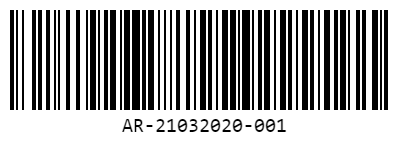
\includegraphics[height=1.5cm]{media/codebarre}\\
		\textbf{\textcolor{vertONE}{ENGLISH}} \\
		
		\vspace*{5pt}
		

		
		\begin{center}
			%%%%%%%%%%%%%%%%%%%%%%%%%%%%
			% Image + cartouche du doc %
			%%%%%%%%%%%%%%%%%%%%%%%%%%%%
			\framebox(479,85){
\includegraphics[height=85pt]{media/banner}}\\
			\vspace{0.3cm}
			%%%%%%%%%%%%%%%%%
			% Cartouche doc %
			%%%%%%%%%%%%%%%%%
			
			\framebox(479,85){ \hfill\begin{minipage}[]{16.5cm}
					\hfill\textbf{\ONEteam}
					\hfill\flushright\large\textbf{\textcolor{bleuONE}{\ONEtitle}}
					\flushright \normalsize \textbf{\hfill \textcolor{gray}{\ONEdate}}
				\end{minipage} }
		\end{center}
		%%%%%%%%%%%%%%%%%%%%%%
		% Tableau Written by %
		%%%%%%%%%%%%%%%%%%%%%%
		\framebox(238,85){\begin{minipage}[]{10cm}
				\begin{center}
					Written by :\\
					\ONEauthor
					\vspace{0.5cm}
					
				\end{center}
				
				
				
		\end{minipage}}
	%%%%%%%%%%%%%%%%%%%%%%%%%%
	% Tableau Date signature %
	%%%%%%%%%%%%%%%%%%%%%%%%%%
	\framebox(238,85){\begin{minipage}[]{10cm}
			\begin{center}
				Date and signature :\\
				\vspace{1cm}
			
			
		\end{center}
			
	\end{minipage}}
\noindent
	%%%%%%%%%%%%%%%%%%%%%%
	% Tableau Checked by %
	%%%%%%%%%%%%%%%%%%%%%%
	\framebox(238,85){\begin{minipage}[]{10cm}
			\begin{center}
				Checked  by :\\
				\ONEchecker
				\vspace{0.5cm}
				
			\end{center}
			
			
			
	\end{minipage}}
	%%%%%%%%%%%%%%%%%%%%%%%%%%
	% Tableau Date signature %
	%%%%%%%%%%%%%%%%%%%%%%%%%%
	\framebox(238,85){\begin{minipage}[]{10cm}
			\begin{center}
				Date and signature :\\
				\vspace{1cm}
				
				
			\end{center}
			
	\end{minipage}}
\vspace{3pt}
%%%%%%%%%%%%%%%%%
% ZONE DE LOGOS %
%%%%%%%%%%%%%%%%%
\begin{center}
	
\includegraphics[height=2.15cm]{media/ipsa} \qquad
	
\includegraphics[height=2.15cm]{media/logooneblack}\qquad
	
\includegraphics[height=2.15cm]{media/logoionis}\\
	
\includegraphics[height=2.15cm]{media/sodern}\qquad
	
\includegraphics[height=2.15cm]{media/icare}
\end{center}
		%%%%%%%%%%%%%%%%%%%%%%%%
		% Footer page de garde %
		%%%%%%%%%%%%%%%%%%%%%%%%
		\begin{center}
			\footnotesize
			\textbf{O}rbital \textbf{N}ano \textbf{E}xperiments\\
			Association Law 1901 hosted at Institut Polytechnique des Sciences Avancées\\
			63 boulevard de Brandebourg – 94200 Ivry-Sur-Seine\\
			Mail : ipsa-one@ipsa.fr
		\end{center}
	\newpage
	
	
	%%%%%%%%%%%%%%%%%%%
	% Page change log %
	%%%%%%%%%%%%%%%%%%%
	\pagestyle{changelog}   % activate colored margins
	\hfill
\includegraphics[height=2cm]{media/logooneblack}
	\begin{center}
		\textbf{\Large CHANGE LOG}
		\vspace{1cm}
		
		\ONEedits
	\end{center}
	
	
	\tableofcontents
	\clearpage
	
	\pagestyle{plain}
	
	\part{introduction}
	\section{Purpose}
	The purpose of this document is to write the specification and software requirement for the on board computer of Arogat-1 cubesat. It provide answer to developer to know what should the system do and not do.
	\section{Acronyms}
	\noindent{\textcolor{black}{
	% Ajouter du texte ici 
\begin{large}
    ADCS\tabto{2cm}Attitude Determination and Control System\\
    CCSDC\tabto{2cm}Consultative Committee for Space Data Systems\\
    CFDP\tabto{2cm}CCSDS File Delivery Protocol\\
    COM\tabto{2cm}Communication\\
    EPS\tabto{2cm}Electrical Power Supply\\
    OBC\tabto{2cm}On Board Computer\\
    TCP\tabto{2cm}Transmission Control Protocol\\
    \end{large}
	}}\hfill
	\newpage 
	
	\section{Reference}
\noindent{\textcolor{black}{
	{[1]} CFDP CCSDS report: \url{https://public.ccsds.org/Pubs/727x0b4.pdf}\\
	\\
    {[2]} TCP summary: \url{https://www.ietf.org/rfc/rfc1594.txt}\\
\\
    {[3]} IP over CCSDS CCSDS report: \url{https://public.ccsds.org/Pubs/702x1b1c1.pdf}\\
\\
    {[4]} Encapsulation Service CCSDS report: \url{https://public.ccsds.org/Pubs/133x1b2c2.pdf}\\
\\
    {[5]} TM CCSDS report: \url{https://public.ccsds.org/Pubs/130x1g2.pdf}\\
\\
    {[6]} TC CCSDS report: \url{https://public.ccsds.org/Pubs/230x1g2e1.pdf}\\
\\
    {[7]} Specification of AX.25 Protocol: \url{https://www.tapr.org/pdf/AX25.2.2.pdf}\\
\\
    {[8]} Specification from: Preliminary Requirements Review ARAGOSAT-1 (AR-050118-001)\\
\\
    {[9]} Interfaces-Commands compared with Documentation of AAU-Cubesat On Board Computer Software: \url{http://www.space.aau.dk/cubesat/dokumenter/software.pdf}\\
\\
    {[10]} Specification can be compared with QB50 System Requirements and Recommendations, Issue 6: \url{https://www.qb50.eu/index.php/tech-docs/category/QB50_system_requirements_issue_606e0.pdf?download=58:qb50-docs}
}}

		\newpage
	\noindent{\textcolor{black}{
	% Ajouter du texte ici 
\begin{large}
Nomenclature:\\
    ADCS\tabto{2cm}Attitude Determination and Control System\\
    CCSDC\tabto{2cm}Consultative Committee for Space Data Systems\\
    CFDP\tabto{2cm}CCSDS File Delivery Protocol\\
    COM\tabto{2cm}Communication\\
    EPS\tabto{2cm}Electrical Power Supply\\
    OBC\tabto{2cm}On Board Computer\\
    TCP\tabto{2cm}Transmission Control Protocol\\
    \end{large}
	}}\hfill
	\part{Modules}
	\section{OBC}
	
	\noindent{\textcolor{black}{
	% Ajouter du texte ici 
	The OBC (On-Board Computer) is the brain of the cubesat. His role is to coordinate all of the other modules and the ground, and also take care of the potential errors and threats for the cubesat. It will periodically (The time interval will depend on the type of data and must be determined individually) send commands to the different critical modules to order them to send critical data (like battery charge for the EPS or spatial orientation for the ADCS). It is absolutely vital for the success of the mission. OBC module shall respect the following requirement: \\
	\\
	\textbf{OBC 1.1 OBC shall collect all Housekeeping data periodically for the entire duration of the mission. Those Data are: Time, the mode, position in space, battery bus voltage, entry voltage of every module, exit voltage from solar panels, engine temperature, engine actual thrust.}\\
	\\
	The period will be determined in the testing process depending on our memory and how many Data can we collect until a downlink.\\
	\\
	\textbf{OBC 1.2 This Data shall be stored in memory until a successful downlink send them to ground.\\
	\\
    OBC 1.3 OBC shall be protected against infinite loop or other kind of Freeze}\\
    \\
    For that we will use Watchdog that are timer that send periodically a ping to the OBC. If the OBC do not respond in time it will be restart. For this we will use real time to be sure that the OBC respect the deadline from the Watchdog except in case of infinite loop or another freeze.\\
    \\
    \textbf{OBC 1.4 OBC shall not override hardware inhibits like deployment switch, remove before flight. [8]\\
    \\
    OBC 1.5 The CubeSat shall allow re-programming of the on-board software during processing on ground and during in-orbit operation. [8]\\
    \\
    OBC 1.6 The CubeSat shall allow changing the software configuration in-orbit, through the use of modifiable parameters (software parametrization). [8]\\
    \\}
}}
    \section{EPS}
    \noindent{\textcolor{black}{
	% Ajouter du texte ici 
	The EPS manages the electricity on board. It's stand alone, it works without the OBC, but the OBC can discuss with it throw different command command. \\
	The OBC can read its stats (for example battery charge) and react accordingly. For that the OBC must send periodically a command through a bus (surely an I²C bus or similar bus) and the EPS sends the data back.EPS module shall respect the following requirement:\\
	 \\
	 \textbf{EPS 2.1 The EPS shall be able to provide the voltage necessity of all subsystem in all modes.\\
	 \\
    EPS 2.2 The EPS shall be powered off until the deployment of the cubesat.\\
    \\
    EPS 2.3 ARG1 electrical system design shall not permit the ground charging circuit to energise the satellite systems (load), including flight computer. [8]
}}}\hfill

    \section{ADCS}
    \noindent{\textcolor{black}{
	% Ajouter du texte ici 
	The ADCS is the module which controls the position of the satellite in space (attitude) and also analyses the environment to determine its position in space.\\
	It is very important for our mission because of our payload, we must control the direction of our engine to control our trajectory.ADCS module shall respect the following requirement:\\
	 \\
	 \textbf{ADCS 4.1 Position Data shall be determined and translate between the OBC and the ADCS.\\
	 \\
    ADCS 4.2 ARG1 shall be able to recover from tumbling rates of up to 90 deg/s per axis by stabilising the satellite attitude before initiating nominal operations. [8]
}}}\hfill

    \section{COM}
    	\noindent{\textcolor{black}{
	% Ajouter du texte ici 
	The COM is the module which allows the communication between the ground and the cubesat. 
	The COM is the link between the ground and the cubesat, so all telecommands and data recovery will go through this module. All data will go through 10 protocoles layer (5 for the ground station and 5 for the cubesat). In terms of data rate, the maximum of our antenna is about 9600bits/s (ref ?).\\
	 \\
    \textbf{
	 COM 6.1 The transceiver shall be able to use a secured transmission protocol using Forward Error Correction. [8]\\
	 \\
    COM 6.2 The transceiver shall have a sensibility high enough to receive the GB signal. [8]\\
    \\
    COM 6.3 The antenna shall be able to transmit without a significant power loss in the worst orientation related the ground station. [8]\\
    \\
    COM 6.4 OBC shall try to deploy the antenna periodically until OBC receive the StopAntennaDeployment command from the ground.
    }}}\hfill
    \begin{figure}[h]
        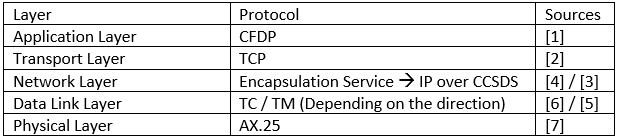
\includegraphics[width=16cm]{media/Protocols Layers COM}
        \caption{Table of the different protocols layers between the ground and the COM}
    \end{figure}
    \section{Engine}
    	\noindent{\textcolor{black}{
	% Ajouter du texte ici 
	The Engine is the payload of our cubesat. His goal is to fight the atmospheric drag to allow the cubesat to have a better life span. \\
	 \\
	 \textbf{
	 \\Engine 7.1 ARG1 Propulsion systems shall have a minimum of three inhibits to its activation.\\
	 \\
    Engine 7.2 ARG1 propulsion system shall remain inhibited until at least TBD minutes after separation.
}
	}}\hfill
	\section{Interfaces}
	\noindent{\textcolor{black}{
	In this part we will see different commands between each modules and the OBC to communicate. This command will surely circulate on I²C bus but it will depend on the commercial hardware that each team will choose.
	}}\hfill
	\begin{figure}[h]
        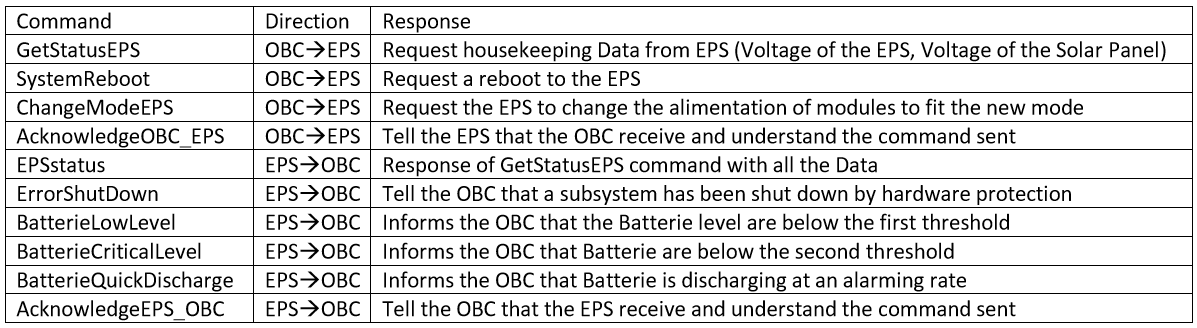
\includegraphics[width=16cm]{InterfaceEpsObc}
        \caption{Interface between OBC and EPS}
    \end{figure}
    \noindent{\textcolor{black}{
    \\
	Values of the two thresholds shall be determined with the simulation.\\
    For the command BatterieQuickDischarge we must be careful that EPS launch it not because of the current mode (For example a massive communication or the Engine at full thrust). Maybe only count unknown consumption.
	}}\hfill
	\begin{figure}[h]
        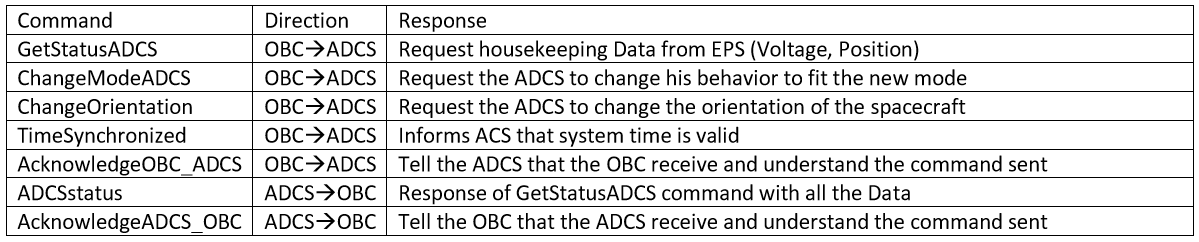
\includegraphics[width=16cm]{InterfaceAdcsObc}
        \caption{Interface between OBC and ADCS}
    \end{figure}
    \begin{figure}[h]
        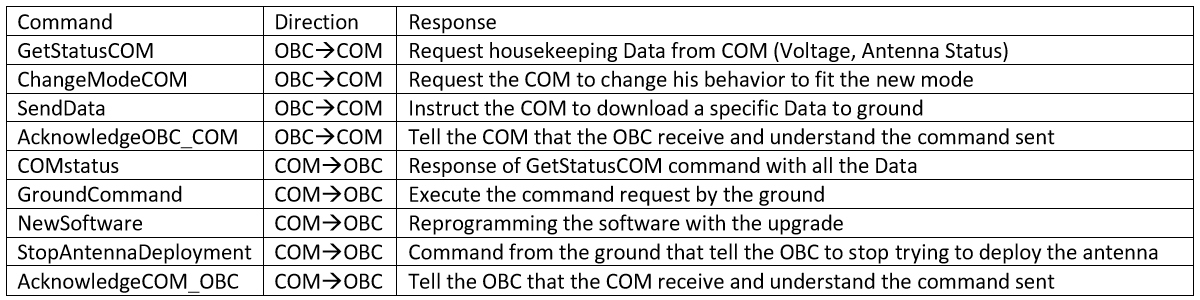
\includegraphics[width=16cm]{InterfaceComObc}
        \caption{Interface between OBC and COM}
    \end{figure}
    \begin{figure}[h]
        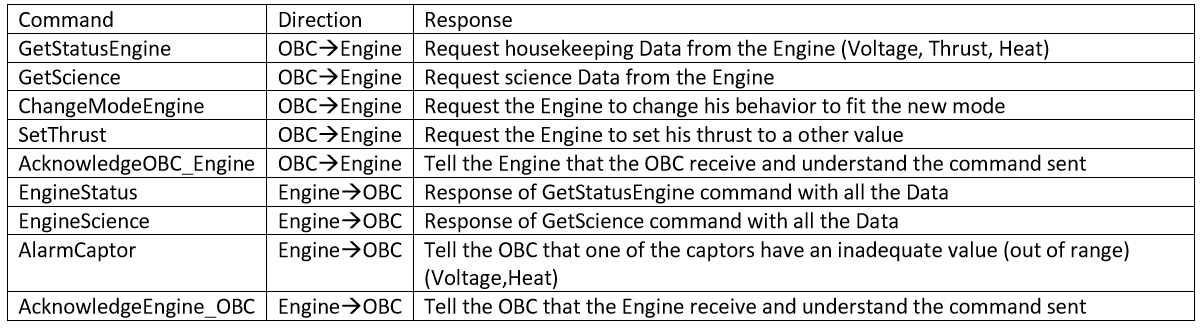
\includegraphics[width=16cm]{InterfaceEngineObc}
        \caption{Interface between OBC and Engine}
    \end{figure}
	
	\part{Modes}
	
	
	\part{Tests Specification}
	
	
	\part{Other Specification}

	
\end{document}